
 
\section{Design Choices} \label{design_choice_android_camera}
In this section I will outline some of the main choices, I faced with during this implementation of my project. I will attempt to outline a balanced view of the options I had and justify my decisions.
 
\subsection{Vision Libraries}
One of the biggest part of the HuddleLamp project is the vision calculations that the computer does. The HuddleLamp project currently uses Opencv as its vision library for different functions such as, calculating the location of the hand of a user and also the location of the mobile devices on the table. In this section I will look at the different vision libraries there are for an Android application.
 
\subsubsection{OpenCV}
The OpenCV (Open Source Computer Vision) is a library that was created to accelerate the adoption of computer vision in application by developers. Some of the mandate for the OpenCV creation was “Advance vision research by providing not only open but also optimised code for basic vision infrastructure. No more reinventing the wheel.”
\cite{opencv_wiki} 
OpenCV is developed in C and C++, however the Applications Interface (API) also includes "wrappers" for Java, MATLAB and Python. There are also community supported ports of Android and iOS platforms.

OpenCV4Android is the official name of the Android port of the OpenCV library. 
\cite{opencv4android_link}. 
Support from NVIDIA towards the project has accelerated the growth of the library for Android. OpenCV4Android allows creation of vision application using OpenCV in 2  different languages.

\cite{opencv_usage_model}. 
\begin{figure}[H]
    \centering
    \begin{subfigure}[b]{0.47\textwidth}
        \centering
        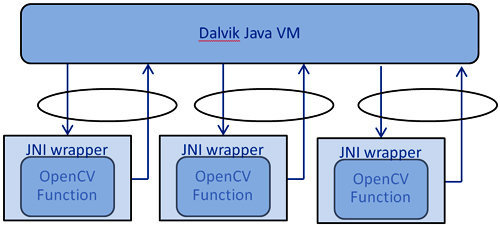
\includegraphics[width=\textwidth]{multiple_jni}
        \caption{An application with Multiple JNI calls}
    \end{subfigure}
    \hfill
    \begin{subfigure}[b]{0.47\textwidth}
        \centering
        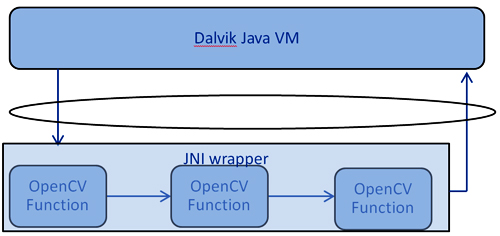
\includegraphics[width=\textwidth]{single_jni}
        \caption{An application with Multiple JNI calls}
    \end{subfigure}
    \hfill
    \caption{A comparison of the 2 usage models\cite{opencv_jni_images}}
     \label{two_usage_models}
\end{figure}

The recommended methods of using OpenCV in Android development is to use the Java API provided with the Software Development Kit SDK\cite{opencv_usage_model}. The learning curve to using the Java API is relatively small. It also has the added advantage of running the program natively, giving you faster processing. However the program calls has the overhead of  one or more Java Native Interface (JNI) calls. There is a JNI call when an OpenCV function starts executing and when it finishes executing. Therefore there will be a large overhead during a complex OpenCV project with multiple calls to the function. Another disadvantage of the Java API is the limited support of the OpenCV C/C++ library.

Another slightly more difficult approach is to use the the Android Native Development Kit (NDK). Android allows native function calls through its NDK, therefore we can use the original C++ interface OpenCV for our application. By encapsulating all the functionality in a single C++ class, we woul only need to call it one per frame, improving the performance of the application. This would also give us access to the whole OpenCV library. Since OpenCV is a cross platform library, this enables me to create a program in a host computer to run and test before porting it to the android device. Figure \ref{two_usage_models} shows the difference between the 2 usage models in terms of JNI calls. 

OpenCV is also the library used by the HuddleLamp group. Which would enable me to replicate their work much easier. However since Android devices does not usually have a Depth Sensor on them, Some aspects of the project needs to be adjusted and compensated differently.

\subsubsection{FastCV}
FastCV is another vision library for mobile devices developed and released by the chip manufacturing giant Qualcomm\cite{fastcv}. It offers developers frequently used computer vision functions that are hardware accelerated. It is a mobile-optimised computer vision (CV) library that used in a wide array of mobile devices.

Figure \ref{opencv_fastcv} shows that FastCV is generally a more optimised library than OpenCV. Almost all the functions are quicker on the FastCV than OpenCV. However FastCV only has a subset of all the functions of OpenCV, which means some functions that might be needed might not be there. It is also a library created and maintained by Qualcomm, subsequently release cycles are less frequent. Open Collaboration of OpenCV means there is more access to underlying architecture and more flexibility in the way to work. 

\begin{figure}[h]
    \centering
    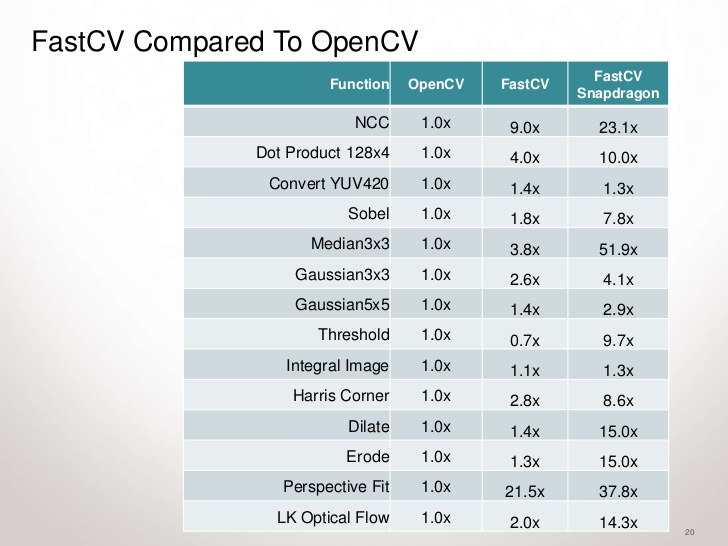
\includegraphics[scale=0.5]{fastcv_opencv}
    \caption{A comparison of the OpenCV vs FastCV \cite{fastcv_opencv}}
    \label{opencv_fastcv}
\end{figure}

FastCV is also only developed for ARM and Qualcomm chipset. Therefore there are devices with Intel and Mips architecture that are not supported and would not be able to run the application.

\subsection{Device Detection} \label{device_identification}

\subsubsection{Glyph Decoding}
Glyph (in typography) is a specific symbol from a set of symbols, intended to be a readable for the purpose of writing\cite{glyph-wiki}. Glyph decoding is the technique used by the HuddleLamp group to identify the devices on the table and its subsequent location\cite{huddlelamp-paper}. By making the devices flash unique symbols on the screen and using the camera application to monitor and detect any of those symbols we are able identify the devices. 

There are some disadvantages to this methods. Primarily the decoding of glyphs would be a resource intensive task because finding a specific symbol on a graphics is quite resource intensive. Also the number of devices that could be used for the table is limited to the number of glyphs in the set of symbols you have. As you increase the set, the memory requirement application would all increase creating potential problems. Creating a Glyph decoding application is also quite difficult due to discrepancies in vision detection as shape detection is quite a difficult task\cite{shape_recognition}.
\subsubsection{Colour Detection}
Another method of detecting the device is to use Colour Detection. Videos are lots of images changing every few milliseconds[wiki]. Images are illustrated as a two dimensional grid of pixels, where pixels contains values to a colour model such as RGB (Red, Green, Blue). We can use this knowledge to detect specific colours from a camera.
By analysing the frames of the video using OpenCV, and making the devices on the table show different unique colours or have coloured marking, we can identify the location of those devices on the table. By looking for large areas of same colour on the images we can identify the devices on the table.


\subsection{Graphics Manipulation}
\subsubsection{Canny edge Detection}
Edge detection is used to filter out information from the images, but still maintaining the structural information about the image that needs to be processed. Edge detection has many uses and has been used for simple object detection to more sophisticated recognition programs\cite{acronym}. Edge detection is quite a hard problem to solve with two main criterion to meet such as edges in the image should not be missed and no spurious responses, the distance between the detected edge and the actual edge should be small\cite{canny-paper}.

One of the more famous edge detection algorithm is called Canny Edge Detection\cite{canny-paper}, named after the person who came up with the algorithm \citeauthor{canny-paper}. Canny edge detection is still a widely used algorithm and very popular in the Computer Vision community. There are 5 main steps in the canny edge detection algorithm\cite{canny-tutorial}.
\begin{enumerate}
\item \textbf{Smoothing}

Most images, taken from a camera, has a lot of noise which could result in spurious results if it is not filtered out. A Gaussian filter is applied to the image to reduce the amount of noise on the image. A Gaussian filter is created by making a convolution mask, smaller than the actual image. The mask is slid over the image, manipulating a square of pixels at a time\cite{canny-tutorial2}. The sobel-operator
\item \textbf{Finding Gradients}

The algorithm finds the edges by finding the locations in the image where the intensity of the grayscale values changes the most. This is achieved through finding the gradients of the image. By applying a \emph{sobel-operator} we are able to determine the gradient\cite{sobel-operator}. Sobel-operator consist of a 3x3 matrix pair, one estimating the gradient in the x- direction and the other estimating the gradient in the y direction. The magnitude of the edge is determined by using a Euclidean distance over the both gradient. The direction of the edge is also determined so that broader detected edges could be thinned.
\item \textbf{Non-Maximum suppression}

The broader edges detected would be thinned by preserving all the local maxima in the gradient image and setting everything else to "0". This is done by rounding the gradient direction to the nearest 45\textdegree and then seeing if that cell is has the biggest value compared to the immediate cell in the positive and the negative gradient. 
\item \textbf{Double thresholding}

The remaining edges after the Non-Maximum suppression could still be due to noise or through colour variation due to rough surfaces. Another way to filter these images more to gain true edges is by thresholding. By setting a threshold value, only the edges stronger than this value would be considered as the true edge. Canny edge Detection does double thresholding where it sets 2 values "strong" and "weak", any edge value bigger than the strong value is considered as a strong edge and lower than "weak"  value is suppressed. Anything in between is marked as a weak edge.
\item \textbf{Edge tracking by hysteresis}

All the strong edges marked from the previous step and automatically added as an edge to the image, and the all the weak edges are only added if they are connected to a strong edge. The reasoning behind is that only proper edge would by higher than the strong threshold values and the weak ones are either due to noise, then they are unlikely to be joined to a strong value or weak due to some colour variation, subject to the values being set proper.
\end{enumerate}

I can use edge detection to determine the location of the devices either through the glyph decoding or through the colour detection method because almost all devices have a black "edge" around the screen of the tablet. By flashing contrasting colours on the screen there would be a definite edge between the screen and the edge which could be detected easily.
\subsubsection{Contours}
Contours are quite similar to edge detection. They are curves that join continuous points along the boundary that has the same colour or intensity\cite{contour-opencv}. The main difference being that the boundaries are joined together to create a line that separate the different colour or intensity unlike edge detection where the points does not have to be joined. Contours are a very useful tool for object detection and recognition as well as shape analysis.

Some of the main features of contours that is available for us through OpenCV is the option to get the area, perimeter etc of the contours\cite{contour-features}. Allowing us to use this information for the object recognition part of out algorithm. Combining contours with gray scaling and colour detection we can easily find objects in the images.




\subsection{Data Storage}
\subsubsection{Firebase}

Firebase\cite{firebase} is a relatively new back-end as a service
company recently acquired by Google. They are a cloud service provider
from San Francisco who caters a number of products for software developers
building mobile or web application. The service we are more interested
is their Real-time Database service. It provides developers with an
API that which enables data to be synchronised across clients automatically
and stored on the Firebase cloud. The main advantage is the fact that
the data gets synchronised within milliseconds. It also supports a
multitude of platforms such as Android, iOS, JavaScript etc.
 
It also only requires client-side code meaning the developers has
a relative easy job to create the back-end they required with. Storing
the information as JSON with every information accessible through
their own URL means the data is easy to store and retrieve and there
is also a readily available rest endpoint.
 
By providing a simple security management system, Firebase ensures
that the data moved through the apps are encrypted and safe. By ensuring
that the security measures are enforced across all parts of the system,
It helps the developer in eradicating glaring security risks. Firebase
built with scaling and performance in mind. When the data changes
Firebase calculates the minimum number of changes required to keep
all the clients in sync. It also scales linearly depending on the
amount of data being synchronised, decreasing the likely hood of a
developer error.
 
The potential of Firebase is enormous. The creators of Firebase hope
that it can serve the needs of 95\% of web service\cite{firebase-wired},
meaning it will be an ideal tool in the stack of our system. One of
its glaring problems is the it is not ideal for processing images,
however the real-time data synchronisation aspect of it make it a
really good candidate for the HuddleTable.
 
 
\subsubsection{Meteor}
 
Meteor\cite{meteor} is a real-time JavaScript framework to come from
the Y-Combinator incubator in 2011. It is primarily used by developers
due to its ability in rapid-prototyping, hence for a MEng project
stack, meteor is an ideal framework to use. It produces cross-platform
code such that for a multiple mobile devices project like HuddleTable
it would cut down on the work required to get most of the devices
to work. It is tightly coupled with the MongoDB, a prominent No-SQL
database. It has an in built publish\textendash subscribe pattern\cite{pub-sub-pattern}
which helps to propagate data changes to clients in real-time without
the need for synchronisation protocols.
 
Some of the design principles used by Meteor makes it a really good
choice for HuddleTable. It has a Data on the wire motivation meaning,
it only sends the minimum data necessary to re-render the portion
of the page that has changed decreasing the latency. It has a full
stack reactivity\cite{meteor-wiki} meaning that everything gets updated
together when required encouraging its simplicity motivation. Its
created in such a way that it is easy to learn and implement even
for beginners.
 
Meteor is the framework of choice used the by HuddleLamp research.
They developed an Object storage on top of Meteor so that all manipulations
on one device become instantly visible on all the other devices. This
allowed the cross platform collaborative work to be done with ease.
Having to only work with one language, JavaScript, on the whole project
means a lot less work for the developer, however the complex algorithm
required for HuddleTable would not be enticing to do in JavaScript.
 
 
\subsubsection{AirDrop / Android Beam}
 
AirDrop\cite{airdrop} is another data sharing service started in
2011 by Apple. It lets you transfer files, links and other content
over the Wi-Fi and Bluetooth between Apple devices. It is a technology
that has been widely appreciated by Apple users and highly congratulated
on. The simple interface to send files back and forth without any
``handshake'' like system and having no restrictions in size of
the files transferred means its a highly appreciated technology which
does not require Internet for it to work. It also has built in function
to control the recipients of the information sent. AirDrop creates
a peer-to-peer Wi-Fi network between the devices and the files are
sent encrypted which means the file transfer is also secure.
 
Android Beam\cite{android-beam} is a similar technology developed
by Android for their devices. It allows android devices to share content
with each other by pressing the devices back to back. Android uses
the Near field Communication (NFC) hardware to transfer the information
between the devices. However compared to the Apple's AirDrop, Android
beam is slower due to it using NFC instead of Wi-Fi. NFC is also not
available on all Android devices.
 
These technologies are restricted because they would only work with
each other. By creating a protocol similar to this which would work
across platform would be an ideal scenario. That would mean that the
devices does not need to be connected to the Internet creating an
opportunity to make an ad-hoc interactive table anywhere.
 

